\documentclass{beamer}
\usetheme{Warsaw}
\usepackage{nhtvslides}
\usepackage{graphicx}
\usepackage{listings}
\lstset{language=CAML,
basicstyle=\ttfamily\footnotesize,
frame=shadowbox,
breaklines=true}
\usepackage[utf8]{inputenc}

\title{Building a physics engine - part 3: collision response}

\author{Dr. Giuseppe Maggiore}

\institute{NHTV University of Applied Sciences \\ 
Breda, Netherlands}

\date{}

\begin{document}
\maketitle

\begin{frame}{Table of contents}
\tableofcontents
\end{frame}

\section{Collision response}
\begin{slide}{Collision response}{Collision response system}{
\item Solving physical constraints in addition to the equations of motion
\item Constraints are mostly contact constraints, but also
\begin{itemize}
\item Friction constraints
\item Distance constraints
\item Joint angle constraints
\item ...
\end{itemize}
\item The ideal collision response system deals with all of these
}\end{slide}

\begin{slide}{Collision response}{Naïve take}{
\item Apply the constraints to the objects in pairs
\item Use the laws of \textit{conservation of motion} for each collision; $P_0$ is the point of collision, $x_A$ and $x_B$ are the centres of mass of the objects, $v^{-1}$ is the pre-impact velocity of the objects, $v^+$ is the post-impact velocity of the objects
\begin{itemize}
\item $f = \frac{-(1 + \epsilon)(N_0 \cdot (v_A^{-1} - v_B^{-1})) + (\omega_A^- \cdot (r_A \times N_0) - \omega_B^- \cdot (r_B \times N_0)))}{1/m_A + 1/m_B + (r_A \times N_0)^T J_A^{-1} (r_A \times N_0) + (r_B \times N_0)^T J_B^{-1} (r_B \times N_0)}$
\item $r_A = P_0 - x_A$, $r_B = P_0 - x_B$
\item $v_A^+ = v_A^- + \frac{f N_0}{m_A}$
\item $\omega_A^+ = \omega_A^- + J_A^- (r_A \times (f N_0))$
\end{itemize}
\item Push away from interpenetration as long as interpenetration exists
}\end{slide}

\begin{slide}{Collision response}{Naïve take}{
\item Jitters a lot, and does not support stacking
\item May be acceptable in very sparse scenarios (space/flight simulator)
}\end{slide}

\begin{slide}{Collision response}{Naïve take number 2}{
\item Apply the constraints to the objects in pairs
\item Apply again during the same tick
\item Average/combine the various impulses
\item Push apart objects so they do not penetrate
\pause
\item Constraints are still broken
\item \textit{Hack-y method}, gives no guarantees
\item Still does not support stacking
}\end{slide}

\section{Constrained dynamics}
\begin{slide}{Constrained dynamics}{Unconstrained kinematics}{
\item A rigid body is characterised by
\item $\dot x = v$
\item $\dot q = \frac{1}{2}wq$
}\end{slide}

\begin{slide}{Constrained dynamics}{Unconstrained kinematics}{
\item For a system of $N$ bodies, we can define the system derivative as
$$V = \left[ \begin{matrix}
v_1 \\ \omega_1 \\ \vdots \\ v_N \\ \omega_N
\end{matrix} \right]$$
}\end{slide}

\begin{slide}{Constrained dynamics}{Constraints}{
\item Our system allows \textit{pairwise} constraints between bodies
\item The $k$-th constraint, between bodies $i$ and $j$, has the form $C_k(x_i,q_i,x_j,q_j) = 0$
\item The vector $C$ holds all the constraints. $C = 0$, or $C(x) = 0$, is a function of the state vector, so by the chain rule $\dot C = J V = 0$
}\end{slide}

\begin{slide}{Constrained dynamics}{Constraint forces}{
\item Each constraint causes a reaction force $f_c$ and a reaction torque $\tau_c$
\item The vector of all reaction forces is $$F_c = \left[ \begin{matrix}
f_{c1} \\ \tau_{c1} \\ \vdots \\ f_{cN} \\ \tau_{cN}
\end{matrix} \right]$$
}\end{slide}

\begin{slide}{Constrained dynamics}{Constraint forces}{
\item We know that $\dot C = J V = 0$
\item $J V = \left[ \begin{matrix}
J_1 \cdot V \\ \vdots \\ J_M \cdot V \\
\end{matrix} \right] = 0$
\item This means that $V$ is orthogonal to each row of $J$
}\end{slide}

\begin{slide}{Constrained dynamics}{Constraint forces}{
\item Constraint forces perform no work, so $F_c \cdot V = 0$
}\end{slide}

\begin{frame}{Principle of virtual work}
\center
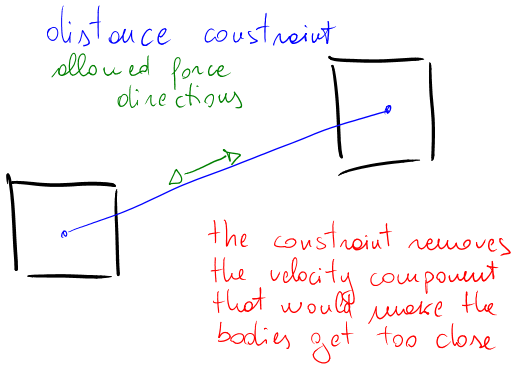
\includegraphics[width=7cm]{Pics/VirtualWork.png}
\end{frame}

\begin{slide}{Constrained dynamics}{Constraint forces}{
\item We can use $F_c = J^T \lambda$ for some vector $\lambda$ of undetermined force multipliers
\item $F_c \cdot V = J^T \lambda \cdot V = (\sum_i J_i \lambda_i) \cdot V = \sum_i J_i \cdot V \lambda_i = \sum_i 0 \lambda_i = 0$
}\end{slide}

\begin{slide}{Constrained dynamics}{Constraint forces}{
\item We will thus compute the matrix $J$ of constraints from the collision system
\item We then solve for $\lambda$, compute $F_c$, and finally obtain $V$
}\end{slide}

\section{Setting up the constraints}
\begin{slide}{Constrained dynamics}{Distance constraints}{
\item The simplest constraint is a distance constraint
\item Two points of two bodies must remain at a given distance
\item $C(x_i,q_i,x_j,q_j) = \frac{1}{2}(|p_j-p_i|^2 - L^2) = 0$
\item If we derive this, we get $\dot C(x_i,q_i,x_j,q_j) = \underbrace{(p_j-p_i)}_{d}(v_j + \omega_j \times r_j - v_i - \omega_i \times r_i)$
\item We split this into a row for $J$ and a part of $V$:
\item $\dot C(x_i,q_i,x_j,q_j) = \underbrace{\left[ -d^T\ -(r_i \times d)^T\ d^T\ (r_j \times d)^T \right]}_{\text{a row of }J} \underbrace{\left[ v_i\ \omega_i\ v_j\ \omega_j \right]^T}_{\text{some columns of } V}$
}\end{slide}

\begin{frame}{Distance constraint}
\center
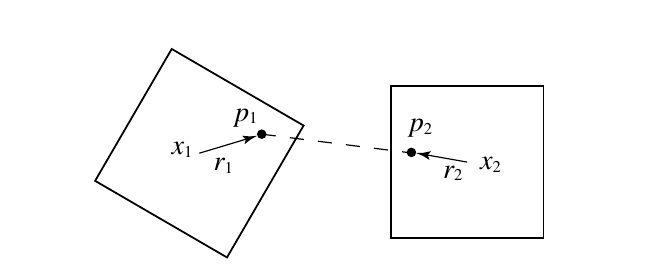
\includegraphics[width=7cm]{Pics/DistanceConstraint.png}
\end{frame}

\begin{slide}{Constrained dynamics}{Distance constraints}{
\item We are abusing the notation; the ``row of $J$'' also contains many zeroes $(6 \times (N_{\text{bodies}} - 2))$
\item The only columns that are not zeroed are those corresponding to the bodies $i$ and $j$
\item $\dot C(x_i,q_i,x_j,q_j) = \underbrace{\left[ \dots\ 0\ -d^T\ -(r_i \times d)^T\ 0\ \dots\ 0\ d^T\ (r_j \times d)^T\ \dots\ 0\right]}_{\text{a row of }J} V$
}\end{slide}

\begin{slide}{Constrained dynamics}{Contact constraints}{
\item We may also model contact constraints
\item The contact constraint measures the object separation; it is negative in case of overlap
\item $C(x_i,q_i,x_j,q_j) = (x_j + r_j - x_i - r_i) \cdot n_i = 0$
\item $\dot C(x_i,q_i,x_j,q_j) = (v_j + \omega_j \times r_j - v_i - \omega_i \times r_i) \cdot n_i + (x_j + r_j - x_i - r_i) \cdot \omega_i \times n_i$
\item We assume that both penetration and angular velocity are small, so we ignore the second term
\item $\dot C(x_i,q_i,x_j,q_j) \approx (v_j + \omega_j \times r_j - v_i - \omega_i \times r_i) \cdot n_i$
}\end{slide}

\begin{frame}{Contact constraint}
\center
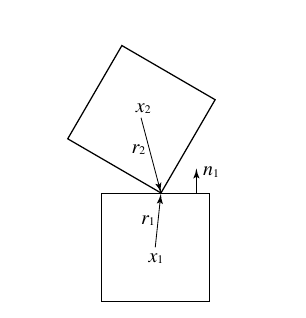
\includegraphics[height=5cm]{Pics/ContactConstraint.png}
\end{frame}

\begin{slide}{Constrained dynamics}{Contact constraints}{
\item We can now separate $\dot C$ into $J$ and $V$:
\item $\dot C(x_i,q_i,x_j,q_j) = (v_j + \omega_j \times r_j - v_i - \omega_i \times r_i) \cdot n_i = \left[ -n_i^T\ -(r_i \times n_i)^T\ n_i^T\ (r_j \times n_i)^T\ \right] \left[ v_i\ \omega_i\ v_j\ \omega_j \right]^T$
}\end{slide}

\begin{slide}{Constrained dynamics}{Contact constraints}{
\item Notice that the force between bodies in contact can push them apart, but not pull them together
\item This means that $0 \leq \lambda_k \leq +\infty$, where $k$ is the constraint index for a contact constraint
}\end{slide}

\begin{slide}{Constrained dynamics}{Contact constraints}{
\item In some cases penetration might happen anyway
\item Numerical errors or issues with discrete steps
\item We allow the velocity to be augmented with a \textit{pushing factor} which is proportional to the penetration
\item This means that for contact constraints $J_i V = -\ \beta C_i$, for $\beta \leq \frac{1}{\Delta t}$
}\end{slide}

\begin{slide}{Constrained dynamics}{Friction constraints}{
\item Friction constraints are very similar to contact constraints
\item Friction happens along the tangent plane, so we have two constraints (one for $u_i = T$ and one for $u_j = B$)
\begin{itemize}
\item $\dot C_{u_i}(x_i,q_i,x_j,q_j) = (v_j + \omega_j \times r_j - v_i - \omega_i \times r_i) \cdot u_i = \left[ -u_i^T\ -(r_i \times u_i)^T\ u_i^T\ (r_j \times u_i)^T\ \right] \left[ v_i\ \omega_i\ v_j\ \omega_j \right]^T$ 
\item $\dot C_{u_j}(x_i,q_i,x_j,q_j) = (v_j + \omega_j \times r_j - v_i - \omega_i \times r_i) \cdot u_j = \left[ -u_j^T\ -(r_i \times u_j)^T\ u_j^T\ (r_j \times u_j)^T\ \right] \left[ v_i\ \omega_i\ v_j\ \omega_j \right]^T$
\end{itemize}
}\end{slide}

\begin{slide}{Constrained dynamics}{Friction constraints}{
\item We must also bound the friction value (this is an approximation) to take the friction coefficient into account
\item $-\mu m_c g \leq \lambda_{u_1} \leq \mu m_c g$ and $-\mu m_c g \leq \lambda_{u_2} \leq \mu m_c g$, where $m_c$ is the mass assigned to the contact point
}\end{slide}

\section{Equations of motion}
\begin{slide}{Equations of motion}{Equations of motion}{
\item We now integrate our constraint system with the equations of motion
\item We know the $Newton-Euler$ equations of motion are 
$\begin{matrix}
m \dot v & = & F & = & f_c + f_{\text{ext}} \\
I \dot w & = & \tau & = & \tau_c + \tau_{\text{ext}} \\
\end{matrix}$
}\end{slide}

\begin{slide}{Equations of motion}{Equations of motion}{
\item We can define a single, big matrix for all the bodies 
$M = \left( \begin{matrix}
m_1 E _{3 \times 3} & 0 & \dots & 0 & 0  \\
0 & I_1 & \dots & 0 & 0  \\
\vdots & \vdots & \ddots & \vdots & \vdots \\
0 & \dots & 0 & m_n E _{3 \times 3} & 0  \\
0 & \dots & 0 & 0 & I_n \\
\end{matrix} \right)$
\item $E_{3 \times 3}$ is just the identity matrix
}\end{slide}

\begin{slide}{Equations of motion}{Equations of motion}{
\item We can easily invert this matrix
$M^{-1} = \left( \begin{matrix}
(m_1 E _{3 \times 3})^{-1} & 0 & \dots & 0 & 0  \\
0 & I_1^{-1} & \dots & 0 & 0  \\
\vdots & \vdots & \ddots & \vdots & \vdots \\
0 & \dots & 0 & (m_n E _{3 \times 3})^{-1} & 0  \\
0 & \dots & 0 & 0 & I_n^{-1} \\
\end{matrix} \right)$
}\end{slide}

\begin{slide}{Equations of motion}{Equations of motion}{
\item We can define a single, big vector for all the external forces 
$F_{\text{ext}} = \left[ \begin{matrix}
f_{\text{ext}1} \\
\tau_{\text{ext}1} \\
\vdots \\
f_{\text{ext}N} \\
\tau_{\text{ext}N} \\
\end{matrix} \right]$
}\end{slide}

\begin{slide}{Equations of motion}{Equations of motion}{
\item Since we know that $F_C = J^T \lambda$, we can rewrite the equations of motion for $n$ bodies as
$\left\{ \begin{matrix}
M \dot V & = & J^T \lambda + F_{\text{ext}} \\
JV & = & \epsilon \\
\end{matrix} \right.$
\item $\epsilon$ is the vector of force offsets which allows contact forces to perform work
\item We have too many unknowns: $V$, $\dot V$, and $\lambda$
}\end{slide}

\begin{slide}{Equations of motion}{Equations of motion}{
\item We approximate $\dot V \approx \frac{V_2 - V_1}{\Delta t}$
\item We replace $\dot V$
$\left\{\begin{matrix}
M \frac{V_2 - V_1}{\Delta t} & = & J^T \lambda + F_{\text{ext}} \\
JV_2 & = & \epsilon \\
\end{matrix} \right.$
\item We solve for $V_2$
$\left\{ \begin{matrix}
V_2 & = & \Delta t M^{-1}(J^T \lambda + F_{\text{ext}}) + V_1\\
V_2 & = & J^T \epsilon
\end{matrix} \right.$
}\end{slide}

\begin{slide}{Equations of motion}{Equations of motion}{
\item We can now finish solving for $\lambda$
\item $J^T \epsilon = \Delta t M^{-1}(J^T \lambda + F_{\text{ext}}) + V_1$
\item $J^T \epsilon - V_1 - \Delta t M^{-1}F_{\text{ext}} = \Delta t M^{-1}(J^T \lambda)$
\item $\frac{\epsilon}{\Delta t} - J V_1 - \Delta t J M^{-1}F_{\text{ext}} = J M^{-1} J^T \lambda$
}\end{slide}

\begin{slide}{Equations of motion}{Equations of motion}{
\item The equation $\frac{\epsilon}{\Delta t} - J V_1 - \Delta t J M^{-1}F_{\text{ext}} = J M^{-1} J^T \lambda$ admits infinite solutions; this is due to redundant constraints, such as a table with more than three legs
\item The force combinations that solve the system are usually infinite
}\end{slide}

\begin{slide}{Equations of motion}{Equations of motion}{
\item Once $\lambda$ is computed, we can determine $F_c$, $F$, and then $V_2$
\item A regular integration step is then performed with the new velocities $V_2$
}\end{slide}

\section{Iterative solution of a system of equations}
\begin{slide}{Iterative solution}{System of equations}{
\item The equation $\frac{\epsilon}{\Delta t} - J V_1 - \Delta t J M^{-1}F_{\text{ext}} = J M^{-1} J^T \lambda$ can be restated in simpler form
\item $\underbrace{\frac{\epsilon}{\Delta t} - J V_1 - \Delta t J M^{-1}F_{\text{ext}}}_{b} = \underbrace{J M^{-1} J^T}_{A} \underbrace{\lambda}_{x}$
\item $A x = b$ for some $A,b$
\item These systems can be solved iteratively with a method such as Projected Gauss-Seidel (PGS)
}\end{slide}

\begin{frame}[fragile]{(Projected) Gauss-Seidel}
\begin{lstlisting}[mathescape=true]
while not converged
  $\Delta x_i$ = $(b_i - \sum_j a_{ij} x_j) / A_{ii}$
  $x_i$ = clamp$(x_i + \Delta x_i, min_i, max_i)$
\end{lstlisting}
\end{frame}

\begin{slide}{Iterative solution}{Sparse matrices}{
\item Remember that $A$ is going to be very sparse
\item You may optimize the summation $\Delta x_i$ \texttt{=} $(b_i - \sum_j a_{ij} x_j) / A_{ii}$ a lot by ignoring the zero entries of $A$
}\end{slide}

\section{Contact caching}
\begin{slide}{Contact caching}{Contact caching}{
\item PGS is faster the closer the initial $x$ vector is to the solution
\item If we store previous contact points and their $\lambda_i$ values, PGS converges sooner
\item Just be aware of this
\begin{itemize}
\item Also be aware that it is rather hard to build in practice
\item If you attempt it, chances of success may be low
\end{itemize}
}\end{slide}

\section{Assignment}
\begin{slide}{Assignment}{Assignment}{
\item Before the end of next week
\item Group-work archive/video on Natschool or uploaded somewhere else and linked in your report
\item Individual report by each of you on Natschool
\item Build a collision response system that supports collisions between multiple objects
}\end{slide}

\begin{frame}{That's it}
\center
\fontsize{18pt}{7.2}\selectfont
Thank you!
\end{frame}

\end{document}


\begin{slide}{SECTION}{SLIDE}{
\item i
}\end{slide}

\begin{frame}[fragile]{SLIDE}
\begin{lstlisting}
CODE
\end{lstlisting}
\end{frame}

\begin{frame}{SLIDE}
\center
%\includegraphics[height=5cm]{Pics/recursive_multiplier.png}
\end{frame}
